\documentclass[border=15pt]{standalone}
\usepackage{amsmath, amssymb}
\usepackage{tikz}
\usetikzlibrary{arrows.meta}

\definecolor{block0}{HTML}{E53935}
\definecolor{block1}{HTML}{1E88E5}
\definecolor{block2}{HTML}{43A047}
\definecolor{block3}{HTML}{FB8C00}
\definecolor{block4}{HTML}{8E24AA}
\definecolor{block5}{HTML}{00ACC1}
\definecolor{block6}{HTML}{F4511E}

\begin{document}
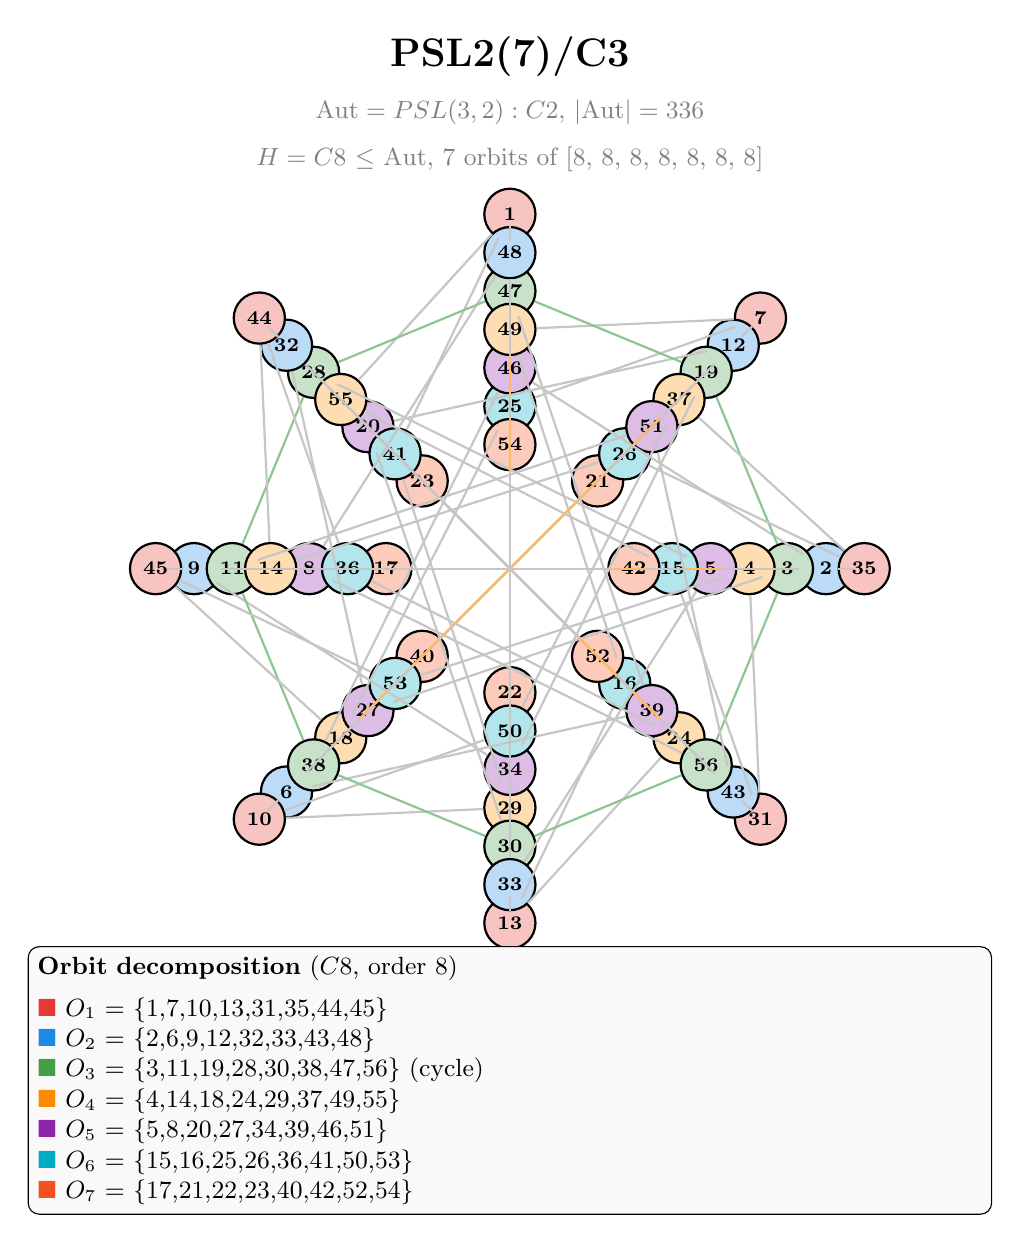
\begin{tikzpicture}[
  vertex/.style={circle, draw, thick, minimum size=6.5mm, inner sep=0pt,
                 font=\scriptsize\bfseries},
  edge/.style={thick, gray!45},
  title/.style={font=\Large\bfseries},
  subtitle/.style={font=\small, text=gray},
]

\node[title] at (0, 6.5) {PSL2(7)/C3};
\node[subtitle] at (0, 5.8) {$\mathrm{Aut} = PSL(3,2) : C2$, $|\mathrm{Aut}| = 336$};
\node[subtitle] at (0, 5.2) {$H = C8$ $\leq$ $\mathrm{Aut}$, 7 orbits of [8, 8, 8, 8, 8, 8, 8]};

\node[vertex, fill=block0!30] (v1) at (0.000, 4.500) {1};
\node[vertex, fill=block1!30] (v2) at (4.013, -0.000) {2};
\node[vertex, fill=block2!30] (v3) at (3.525, -0.000) {3};
\node[vertex, fill=block3!30] (v4) at (3.038, -0.000) {4};
\node[vertex, fill=block4!30] (v5) at (2.550, -0.000) {5};
\node[vertex, fill=block1!30] (v6) at (-2.837, -2.837) {6};
\node[vertex, fill=block0!30] (v7) at (3.182, 3.182) {7};
\node[vertex, fill=block4!30] (v8) at (-2.550, 0.000) {8};
\node[vertex, fill=block1!30] (v9) at (-4.013, 0.000) {9};
\node[vertex, fill=block0!30] (v10) at (-3.182, -3.182) {10};
\node[vertex, fill=block2!30] (v11) at (-3.525, 0.000) {11};
\node[vertex, fill=block1!30] (v12) at (2.837, 2.837) {12};
\node[vertex, fill=block0!30] (v13) at (-0.000, -4.500) {13};
\node[vertex, fill=block3!30] (v14) at (-3.038, 0.000) {14};
\node[vertex, fill=block5!30] (v15) at (2.062, -0.000) {15};
\node[vertex, fill=block5!30] (v16) at (1.458, -1.458) {16};
\node[vertex, fill=block6!30] (v17) at (-1.575, 0.000) {17};
\node[vertex, fill=block3!30] (v18) at (-2.148, -2.148) {18};
\node[vertex, fill=block2!30] (v19) at (2.493, 2.493) {19};
\node[vertex, fill=block4!30] (v20) at (-1.803, 1.803) {20};
\node[vertex, fill=block6!30] (v21) at (1.114, 1.114) {21};
\node[vertex, fill=block6!30] (v22) at (-0.000, -1.575) {22};
\node[vertex, fill=block6!30] (v23) at (-1.114, 1.114) {23};
\node[vertex, fill=block3!30] (v24) at (2.148, -2.148) {24};
\node[vertex, fill=block5!30] (v25) at (0.000, 2.062) {25};
\node[vertex, fill=block5!30] (v26) at (1.458, 1.458) {26};
\node[vertex, fill=block4!30] (v27) at (-1.803, -1.803) {27};
\node[vertex, fill=block2!30] (v28) at (-2.493, 2.493) {28};
\node[vertex, fill=block3!30] (v29) at (-0.000, -3.038) {29};
\node[vertex, fill=block2!30] (v30) at (-0.000, -3.525) {30};
\node[vertex, fill=block0!30] (v31) at (3.182, -3.182) {31};
\node[vertex, fill=block1!30] (v32) at (-2.837, 2.837) {32};
\node[vertex, fill=block1!30] (v33) at (-0.000, -4.013) {33};
\node[vertex, fill=block4!30] (v34) at (-0.000, -2.550) {34};
\node[vertex, fill=block0!30] (v35) at (4.500, -0.000) {35};
\node[vertex, fill=block5!30] (v36) at (-2.062, 0.000) {36};
\node[vertex, fill=block3!30] (v37) at (2.148, 2.148) {37};
\node[vertex, fill=block2!30] (v38) at (-2.493, -2.493) {38};
\node[vertex, fill=block4!30] (v39) at (1.803, -1.803) {39};
\node[vertex, fill=block6!30] (v40) at (-1.114, -1.114) {40};
\node[vertex, fill=block5!30] (v41) at (-1.458, 1.458) {41};
\node[vertex, fill=block6!30] (v42) at (1.575, -0.000) {42};
\node[vertex, fill=block1!30] (v43) at (2.837, -2.837) {43};
\node[vertex, fill=block0!30] (v44) at (-3.182, 3.182) {44};
\node[vertex, fill=block0!30] (v45) at (-4.500, 0.000) {45};
\node[vertex, fill=block4!30] (v46) at (0.000, 2.550) {46};
\node[vertex, fill=block2!30] (v47) at (0.000, 3.525) {47};
\node[vertex, fill=block1!30] (v48) at (0.000, 4.013) {48};
\node[vertex, fill=block3!30] (v49) at (0.000, 3.038) {49};
\node[vertex, fill=block5!30] (v50) at (-0.000, -2.062) {50};
\node[vertex, fill=block4!30] (v51) at (1.803, 1.803) {51};
\node[vertex, fill=block6!30] (v52) at (1.114, -1.114) {52};
\node[vertex, fill=block5!30] (v53) at (-1.458, -1.458) {53};
\node[vertex, fill=block6!30] (v54) at (0.000, 1.575) {54};
\node[vertex, fill=block3!30] (v55) at (-2.148, 2.148) {55};
\node[vertex, fill=block2!30] (v56) at (2.493, -2.493) {56};

\draw[edge] (v1) -- (v41);
\draw[edge] (v1) -- (v48);
\draw[edge] (v1) -- (v55);
\draw[edge] (v2) -- (v17);
\draw[edge] (v2) -- (v35);
\draw[edge] (v2) -- (v46);
\draw[thick, block2!60] (v3) -- (v19);
\draw[edge] (v3) -- (v27);
\draw[thick, block2!60] (v3) -- (v56);
\draw[thick, block3!60] (v4) -- (v14);
\draw[edge] (v4) -- (v31);
\draw[edge] (v4) -- (v53);
\draw[edge] (v5) -- (v28);
\draw[edge] (v5) -- (v33);
\draw[edge] (v5) -- (v42);
\draw[edge] (v6) -- (v10);
\draw[edge] (v6) -- (v21);
\draw[edge] (v6) -- (v39);
\draw[edge] (v7) -- (v12);
\draw[edge] (v7) -- (v25);
\draw[edge] (v7) -- (v49);
\draw[edge] (v8) -- (v17);
\draw[edge] (v8) -- (v48);
\draw[edge] (v8) -- (v56);
\draw[edge] (v9) -- (v34);
\draw[edge] (v9) -- (v42);
\draw[edge] (v9) -- (v45);
\draw[edge] (v10) -- (v29);
\draw[edge] (v10) -- (v50);
\draw[thick, block2!60] (v11) -- (v28);
\draw[thick, block2!60] (v11) -- (v38);
\draw[edge] (v11) -- (v51);
\draw[edge] (v12) -- (v20);
\draw[edge] (v12) -- (v40);
\draw[edge] (v13) -- (v16);
\draw[edge] (v13) -- (v24);
\draw[edge] (v13) -- (v33);
\draw[edge] (v14) -- (v26);
\draw[edge] (v14) -- (v44);
\draw[edge] (v15) -- (v31);
\draw[edge] (v15) -- (v42);
\draw[edge] (v15) -- (v55);
\draw[edge] (v16) -- (v49);
\draw[edge] (v16) -- (v52);
\draw[edge] (v17) -- (v36);
\draw[edge] (v18) -- (v25);
\draw[thick, block3!60] (v18) -- (v37);
\draw[edge] (v18) -- (v45);
\draw[edge] (v19) -- (v34);
\draw[thick, block2!60] (v19) -- (v47);
\draw[edge] (v20) -- (v23);
\draw[edge] (v20) -- (v30);
\draw[edge] (v21) -- (v26);
\draw[edge] (v21) -- (v51);
\draw[edge] (v22) -- (v34);
\draw[edge] (v22) -- (v48);
\draw[edge] (v22) -- (v50);
\draw[edge] (v23) -- (v41);
\draw[edge] (v23) -- (v43);
\draw[edge] (v24) -- (v36);
\draw[thick, block3!60] (v24) -- (v55);
\draw[edge] (v25) -- (v54);
\draw[edge] (v26) -- (v35);
\draw[edge] (v27) -- (v32);
\draw[edge] (v27) -- (v40);
\draw[thick, block2!60] (v28) -- (v47);
\draw[edge] (v29) -- (v41);
\draw[thick, block3!60] (v29) -- (v49);
\draw[thick, block2!60] (v30) -- (v38);
\draw[thick, block2!60] (v30) -- (v56);
\draw[edge] (v31) -- (v43);
\draw[edge] (v32) -- (v44);
\draw[edge] (v32) -- (v52);
\draw[edge] (v33) -- (v54);
\draw[edge] (v35) -- (v37);
\draw[edge] (v36) -- (v44);
\draw[edge] (v37) -- (v50);
\draw[edge] (v38) -- (v46);
\draw[edge] (v39) -- (v47);
\draw[edge] (v39) -- (v52);
\draw[edge] (v40) -- (v53);
\draw[edge] (v43) -- (v51);
\draw[edge] (v45) -- (v53);
\draw[edge] (v46) -- (v54);

\node[draw, rounded corners, fill=gray!5, text width=12cm, align=left, font=\small]
  at (0, -6.5) {
  \textbf{Orbit decomposition} ($C8$, order 8) \\[4pt]
  \textcolor{block0}{$\blacksquare$} $O_{1}$ = \{1,7,10,13,31,35,44,45\} \\
  \textcolor{block1}{$\blacksquare$} $O_{2}$ = \{2,6,9,12,32,33,43,48\} \\
  \textcolor{block2}{$\blacksquare$} $O_{3}$ = \{3,11,19,28,30,38,47,56\} (cycle) \\
  \textcolor{block3}{$\blacksquare$} $O_{4}$ = \{4,14,18,24,29,37,49,55\} \\
  \textcolor{block4}{$\blacksquare$} $O_{5}$ = \{5,8,20,27,34,39,46,51\} \\
  \textcolor{block5}{$\blacksquare$} $O_{6}$ = \{15,16,25,26,36,41,50,53\} \\
  \textcolor{block6}{$\blacksquare$} $O_{7}$ = \{17,21,22,23,40,42,52,54\}
};

\end{tikzpicture}
\end{document}